\documentclass{article}
\usepackage[pdftex]{graphicx}
\begin{document}
\section{Introduction}
This note documents studies and findings regarding various current limiting circuits. 
\section{Analysis of Horowitz and Hill Foldback Scheme}
Horowitz and Hill provide three examples of current protection in association with a voltage regulator and pass transistor.  Focusing on issues of over-current protection, a scheme
evolves that looks like that shown in Figure~\ref{fig:horowitz_and_hill_scheme}.

\begin{figure}[htb]
\begin{center}
%\includegraphics[height=1in,width=1in,angle=-90]
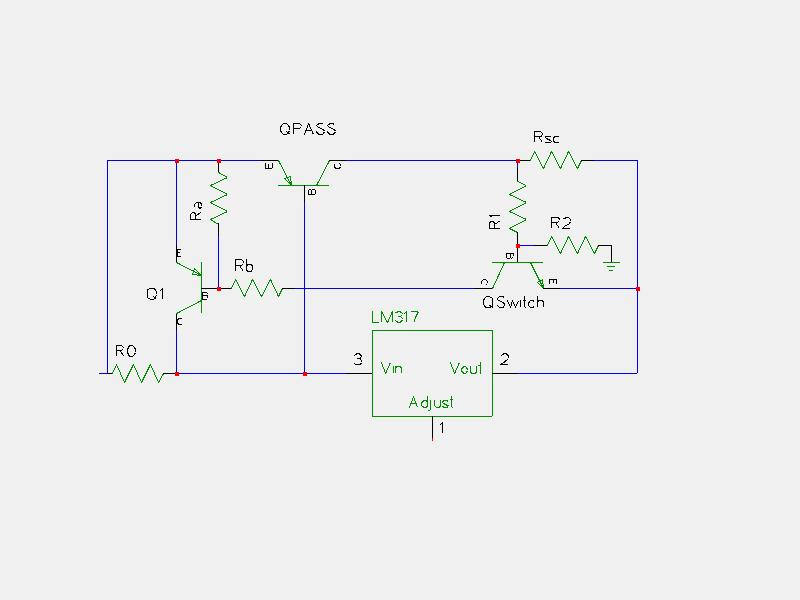
\includegraphics[height=60mm]{Horowitz_Hill_Foldback_Fig5_30B.jpeg}
\caption{Pass transistor configuration discussed by Horowitz and Hill}
\label{fig:horowitz_and_hill_scheme}
\end{center}

\end{figure}

\begin{figure}[htb]
\begin{center}
%\includegraphics[height=1in,width=1in,angle=-90]
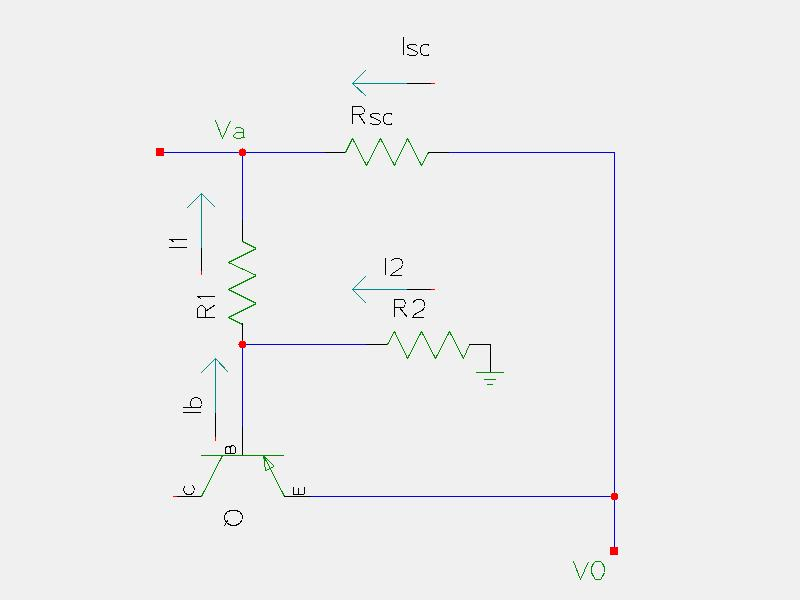
\includegraphics[height=60mm]{foldback_1.jpeg}
\caption{Current protection for pass transistor with foldback.}
\label{fig:foldback-detail-schematic}
\end{center}
\end{figure}

\begin{figure}[htb]
\begin{center}
%\includegraphics[height=1in,width=1in,angle=-90]
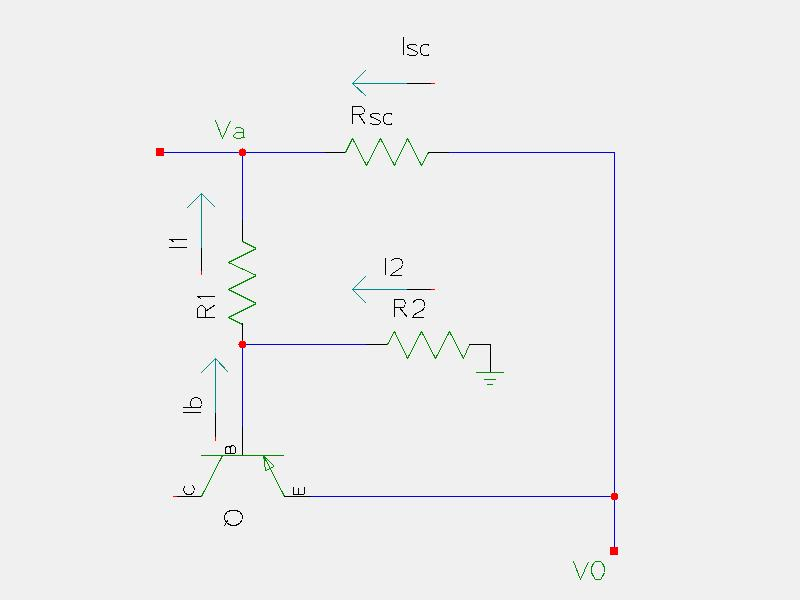
\includegraphics[height=60mm]{foldback_1.jpeg}
\caption{Current protection for pass transistor with foldback.}
\label{fig:predicted-observed}
\end{center}
\end{figure}

The short description provided by Horowitz and Hill turns out to be somewhat misleading as its performance is not as simple as a foldback short-circuit limit of the output current. Instead, it should be regarded as a method of
boosting the current limit of the regulator to a higher value with a
pass transistor and using additional circuitry, including the foldback, to liit the current through the pass transistor-{\it not the output current}.

Briefly, the circuit acts as follows: Resistor $R_0$ is used to control the 
turn-on of the pass transistor. The pass transistor, $Q^{PASS}$ then carries additional current until transistor $Q^{Switch}$ draws current that is used to turn on transistor $Q1$ which diverts additional current back to the regulator. Once the regulator is enabled, transistor $Q^{Switch}$ keeps current through $R_{SC}$ fixed via $V_{BE}$ while the regulator does its work. 
Output voltage and current are then partly determined by the regulator $I-V$ profile. 
A measured profile for an LM337T is shown in 
Figure~\ref{fig:lm337_i_v}. 
Note that once the regulator output voltage begins to drop, the current limit for $I_{SC}$ will also change. Furthermore, the base current for $Q^{Switch}$ becomes non-negligable. This affects the share of the current from the pass transistor. 

Points that were not obvious from a casual reading within Horowitz and Hill:
\begin{itemize}
\item{Although transistor $Q^{PASS}$ is protected, transistor $Q1$ still has to be able to carry the maximum allowed by the regulator.}
\item{The scheme is obviously (in hindsight) not very useful in concocting a supply with an intended limit less than that of the regulator. That is, the circuit provides a limit to the output current equal to the sum of the regulator limit and that imposed by the current protection to the current protection elements}
\item{Detailed expectations can depend sensitively on the degree to which usual assumptions, like ignoring base currents, are ignorable.}
\end{itemize}
With transistor $Q^{Switch}$ on, the current passing through limiting resistor $R_{sc}$ is given by
$$
I_{sc}R_{sc}=
I_b R_1 + 
V_{BE}^{Q^{Switch}} (1+\frac{R_1}{R_2})-
V(\frac{R_1}{R_2}).
$$
The term linear in V is the usual foldback term that brings the current 
down as the voltage drops.
The term proportional to $I_b$ can distort the foldback properties since 
it tends to increase as short circuit conditions are approached. 
Key features of this formalism are 1) The point at which 
the regulator turns on; and 2) 
The short-circuit current. The regulator turn-on is derived by 
setting $I_b = 0$ and $V=V^{nominal}$.


The expression agrees very well with measured configurations. 
See Figure ~\ref{fig:predicted-observed}.
Note that this is due primarily to the increase in the base current driving 
$Q^{Switch}$. The regulator eventually tops out and begins reducing 
output voltage. 
As the regulator maintains roughly its maximum current, $I_{sc}$ drops 
in parallel with $V_o$, so that the curve of $I_{sc}-V_o$ rises 
until the regulator maxes out and drops thereafter 
with the same profile as the current protection provided by the regulator.
In any case, the basic facts are that the circuit does not implement 
any additional foldback. 
The foldback component drives the point at which the regulator 
begins to provide its additional 2 Amps of current. 
Thereafter, the regulator performance drives the behavior of the circuit. 
Examples of values and their features are shown in table ~\ref{Table:examples}.

During testing, one further observation was that during short-circuit 
testing, there was considerable variability in the performance of the circuit. 
Current speculation is that this is due to cooling issues. 
However, it is also likely that the shape of the regulator $I-V$ 
curve for currents above $1.8 \ A$ is likely to make it difficult to
 predict the behavior in this region. In this region, the output 
voltage can vary significantly for very small changes in regulator current. 
There may even be points where the same current is a 'stable' 
operating point for different voltages-the measurement precision 
makes it difficult to be sure of this though.

Determining appropriate values for
 $R_a$ and $R_b$ was difficult. They are unspecified in
the original presentation by Horowitz and Hill.
The values of these transistors can determine
when $Q1$ goes into saturation. 
If $Q1$ is in saturation, the term containing $I_b$ for $I_{sc}$ 
becomes important. Effectively, $I_b \approx 1/\beta ^2$ and $\beta$ becomes 
smaller in saturation. Transistor $Q1$ has to carry 
up to $\approx \ 2 \ A$. 

However, without saturating the transistors, 
I have observed an oscillation in the circuit that I have come to 
suspect is due to the different turn-ons and thresholds for the transistors 
and regulators cannibalizing one another. 
In any event, it commences when $Q^{switch}$ is far 
from saturation (as determined by $V_{ce}$ when the regulator 
first begins to take back current from $Q^{pass}$ and 
it stops when the load current is high enough to saturate $Q^{switch}$. 
Since the minimum current is set by $R_a$, an appropriate value 
for $R_b$ can be estimated by setting $V_c^{Q^{switch}}$ close to $V_{out}$, 
the base of $Q1$ to one diode-drop below $V_{in}$ and using 
$R_a$ to determine the current. Values of $R_a = 100 \O$ and $R_b=1470$ 
seem reasonable. With these values, however, the base 
current for $Q^{switch}$ can rise to 100 mA for a 
load current of $\sim 4 \ A$ which will provide an overall 
current limit of around $4 \ A$ (assuming a limit of $\sim 2 \ A$ 
for the regulator. 
Limiting the pass transistor to less than this with this circuit is 
very difficult.

 Frustrated with the existence of the ringing behavior, I suspected 
it may have been connected to comments in the literature for the 
LM317 regulators on the need for filter capacitors. 
Placement of capacitors along those suggested locations 
did not solve the behavior, but motivated by it, 
I placed a filter capacitor at the collector to 
$Q^{switch}$ and it appears to have cured the ringing.

With this arrangement, 
I was able to arrive at reasonably clean I-V curves 
for the pass, output, and regulator currents. 
These are shown in Figure ~\ref{fig:foldbacks}. Notice that
for two configurations, the foldback curve is exactly as expected.
One configuration shows obvious effects from saturating $Q^{switch}$
and one is marginally saturating.
\begin{figure}[htb]
\begin{center}
%\includegraphics[height=1in,width=1in,angle=-90]
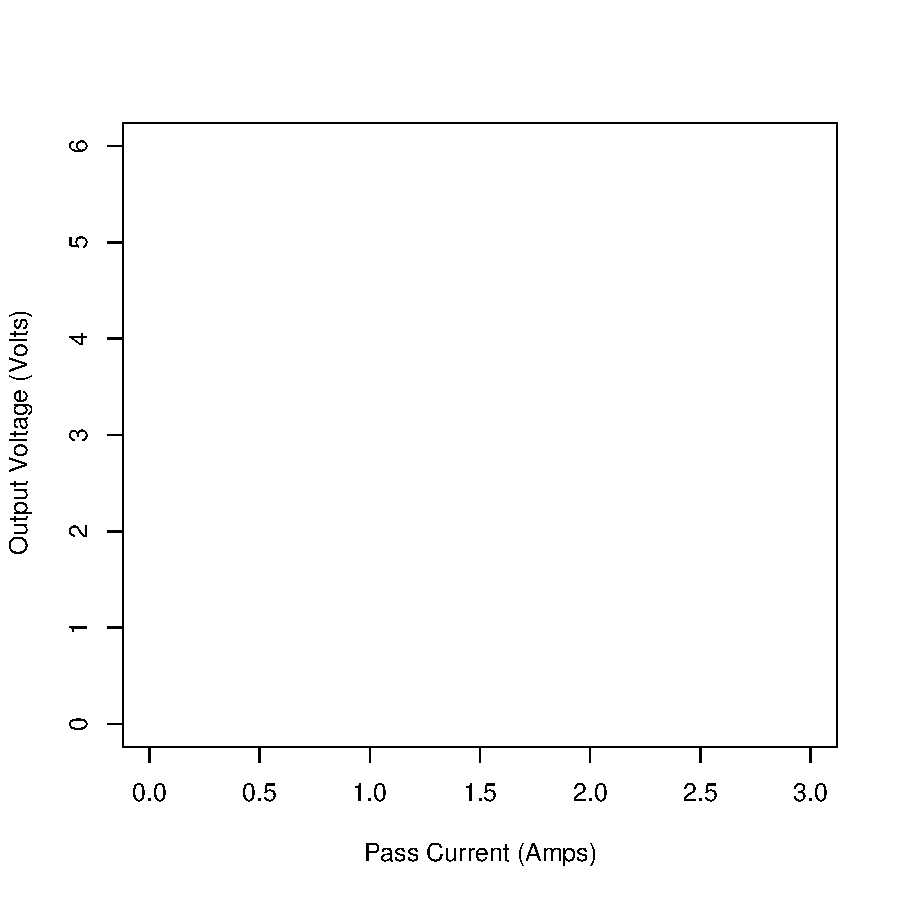
\includegraphics[height=60mm]{pass_current_vs_vout.pdf}
\caption{Measured I-V curves for pass transistor}
\label{fig:foldbacks}
\end{center}

\end{figure}


Having removed the ringing, criteria for selecting $R_a$ and $R_b$ derive from 
avoiding saturation of the switch transistor. 
Again, saturation of this transistor will boost the base current to levels 
that will affect the pass current. 
Avoiding saturation means that $R_b$ should be small enough so that the base current of $Q_1$ 
adds a small drop ($i_b^{Q_1} R_b$ should be 'small') and the drop accross $R_a$ and $R_b$, 
approximately $V_{be} \frac{R_a+R_b}{R_a}$,  
should be less than the difference between $V_{in}$ and $V_{out}$. 
Otherwise, $Q_{switch}$ collector will approach $V_{out}$ and saturate.  
\end{document}
